\documentclass[12pt]{article}
\usepackage[utf8]{inputenc}
\usepackage{graphicx} % Allows you to insert figures
\usepackage{amsmath} % Allows you to do equations
\usepackage{fancyhdr} % Formats the header
\usepackage{geometry} % Formats the paper size, orientation, and margins
\linespread{1.25} % about 1.5 spacing in Word
\setlength{\parindent}{0pt} % no paragraph indents
\setlength{\parskip}{1em} % paragraphs separated by one line
\usepackage[format=plain,
            font=it]{caption} % Italicizes figure captions
\usepackage[english]{babel}
\usepackage{csquotes}
\renewcommand{\headrulewidth}{0pt}
\geometry{letterpaper, portrait, margin=1in}
\setlength{\headheight}{14.49998pt}

\newcommand\titleofdoc{\LARGE{\textbf{Assignment-9: Spectra of Non-Periodic signals}}}
\newcommand\GroupName{EE20B136}

\begin{document}
\begin{titlepage}
   \begin{center}
        \vspace*{4cm} % Adjust spacings to ensure the title page is generally filled with text

        \Huge{\titleofdoc} 

        \vspace{3 cm}
        \Large{Syam SriBalaji T}
       
        \vspace{0.25cm}
        \large{EE20B136}
       
        \vspace{3 cm}
        \Large{May 11, 2022}
        
        \vspace{0.25 cm}
        \Large{EE2703: Jan-May 2022}
       

       \vfill
    \end{center}
\end{titlepage}

\setcounter{page}{2}
\pagestyle{fancy}
\fancyhf{}
\rhead{\thepage}


\newpage
\section*{Introduction:}
In this assignment, we will proceed further with our discussion on Fourier transform. Here, we will be working on Non-Periodic signals. The concepts we will be going through now are-
\begin{itemize}
  \item Plot DFT of Non-Periodic functions
  \item Improvise it with Hamming Window
  \item Fit sinusoidal to Windowed signal and extract its frequency and phase
  \item Analyze the same for noised signal
  \item Work with Chirped signal and plot its Magnitude and Phase surface plot
\end{itemize}

\section*{Question: 1}
Here is the Spectrum of $\sin(\sqrt{2}t)$ in frequency domain-
\begin{figure}[h!]
\centering
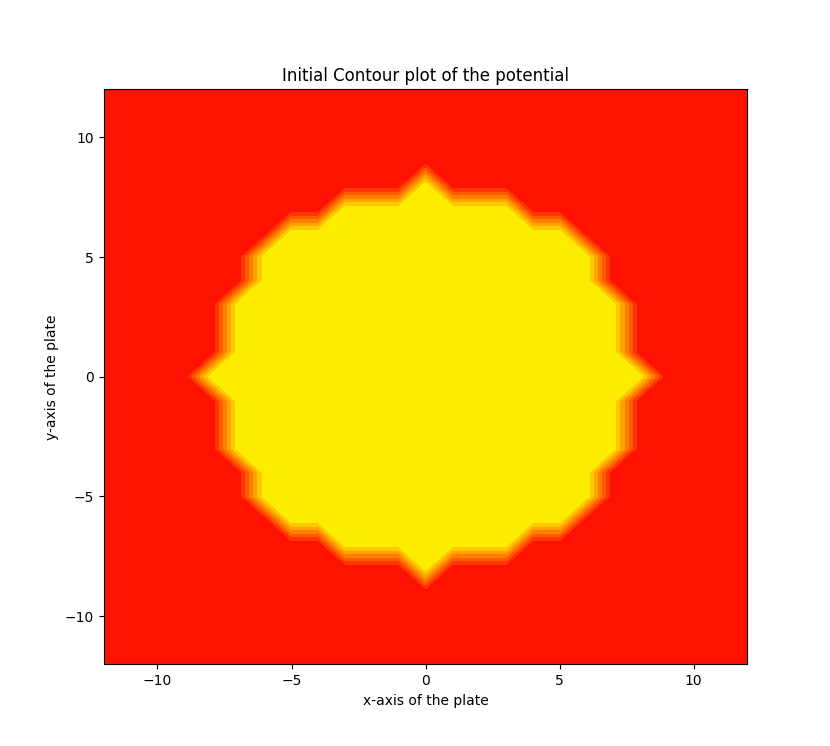
\includegraphics[height=10cm]{Figure_1.png}
\label{fig:exemplo}
\end{figure}

\newpage
Here is the plot of $\sin(\sqrt{2}t)$ time domain-
\begin{figure}[h!]
\centering
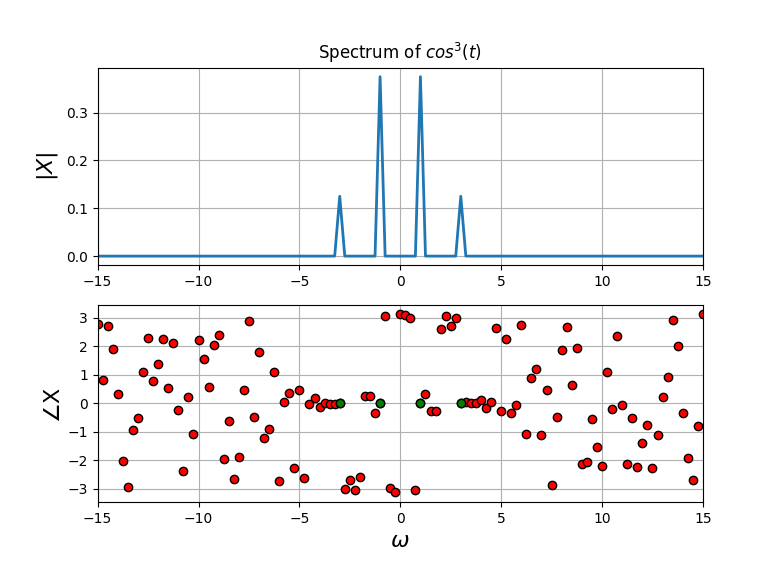
\includegraphics[height=9cm]{Figure_2.png}
\label{fig:exemplo}
\end{figure}

As we need the DFT over a finite time interval. We here plot the DFT of the above function in $(-\pi,\pi)$ interval
\begin{figure}[h!]
\centering
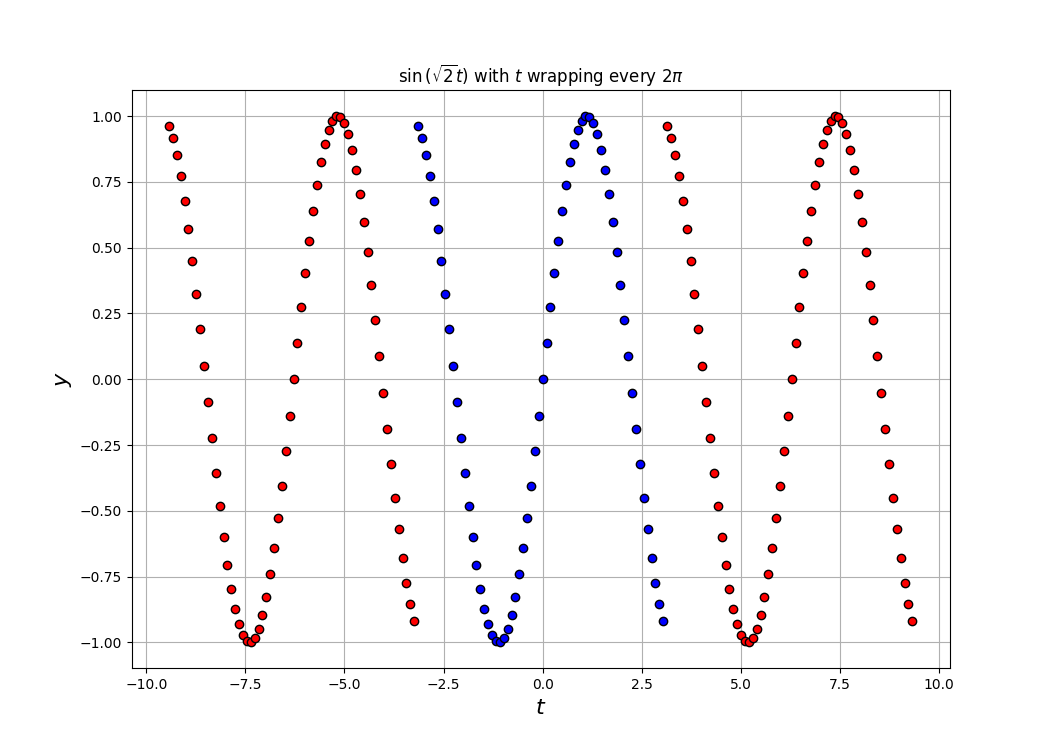
\includegraphics[height=9cm]{Figure_3.png}
\label{fig:exemplo}
\end{figure}

\newpage
As we can see in the above plot, the big jumps at n$\pi$ will lead to Non-harmonic components in FFT, and cause slow decaying with $\frac{1}{\omega}$. To verify this we will be plotting periodic ramp of it.

\begin{figure}[h!]
\centering
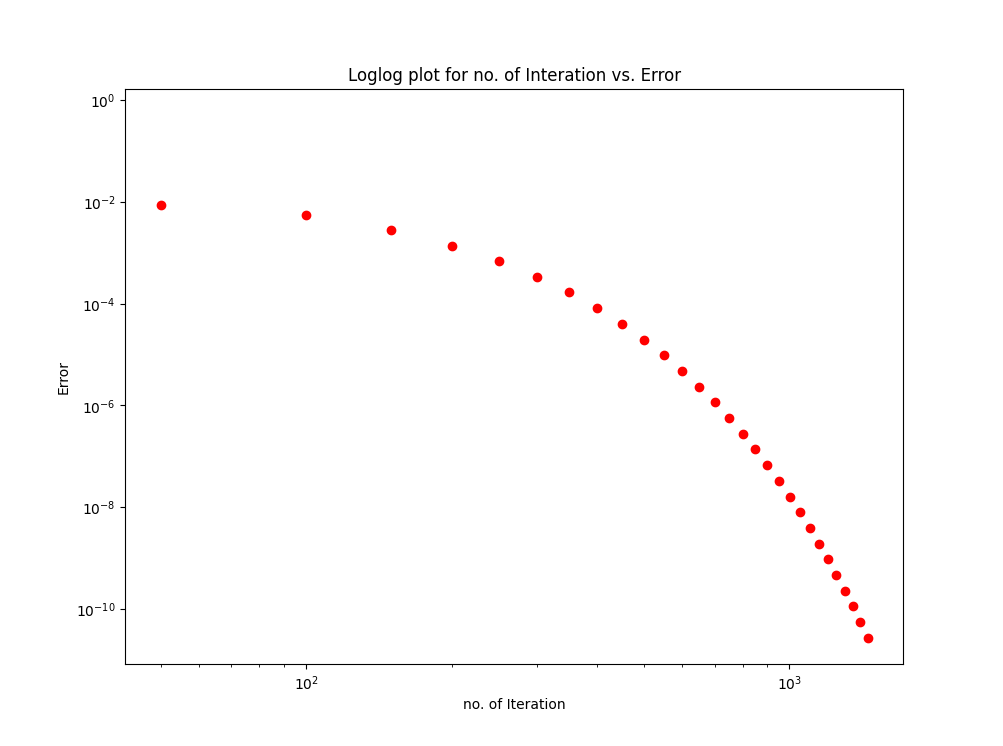
\includegraphics[height=11cm]{Figure_4.png}
\label{fig:exemplo}
\end{figure}

From here we confirm the presence of discontinuities. This is why we need Hamming window.

\newpage
\section*{Windowing:}
The hamming window removes the discontinuities by attenuating the high frequency components in DFT of $\sin(\sqrt{2}t)$. The hamming window given is-

  \begin{equation}
    \omega[n]=
    \begin{cases}
      0.54+0.46\times cos(\frac{2\pi n}{N-1}) & \text{for } |n|\leq\frac{N-1}{2} \\
      0  & \text{else } 
    \end{cases}
  \end{equation}
  
We will multiply this hamming window function to DFT of $\sin(\sqrt{2}t)$, we get-  
\begin{figure}[h!]
\centering
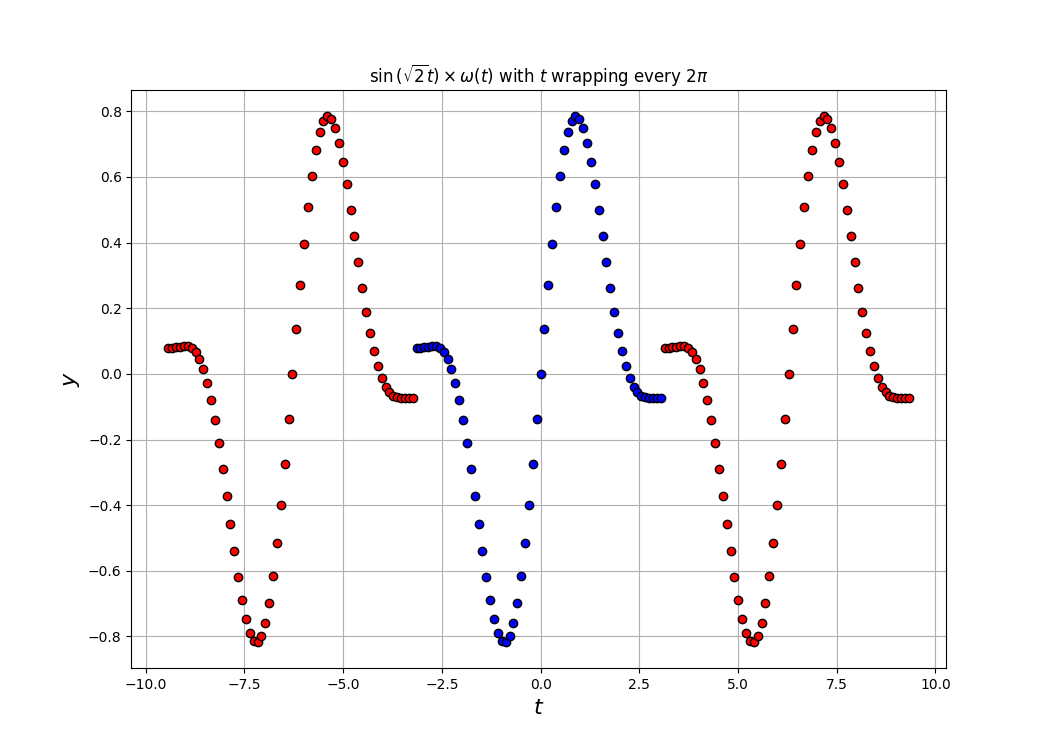
\includegraphics[height=12cm]{Figure_5.png}
\label{fig:exemplo}
\end{figure}

Now, we can see the jump (i.e. discontinuities) is very decreased. So we can proceed to do DFT of $\sin(\sqrt{2}t)$.

\newpage
This is the spectrum of $\sin(\sqrt{2}t)$ with time period $2\pi$-

\begin{figure}[h!]
\centering
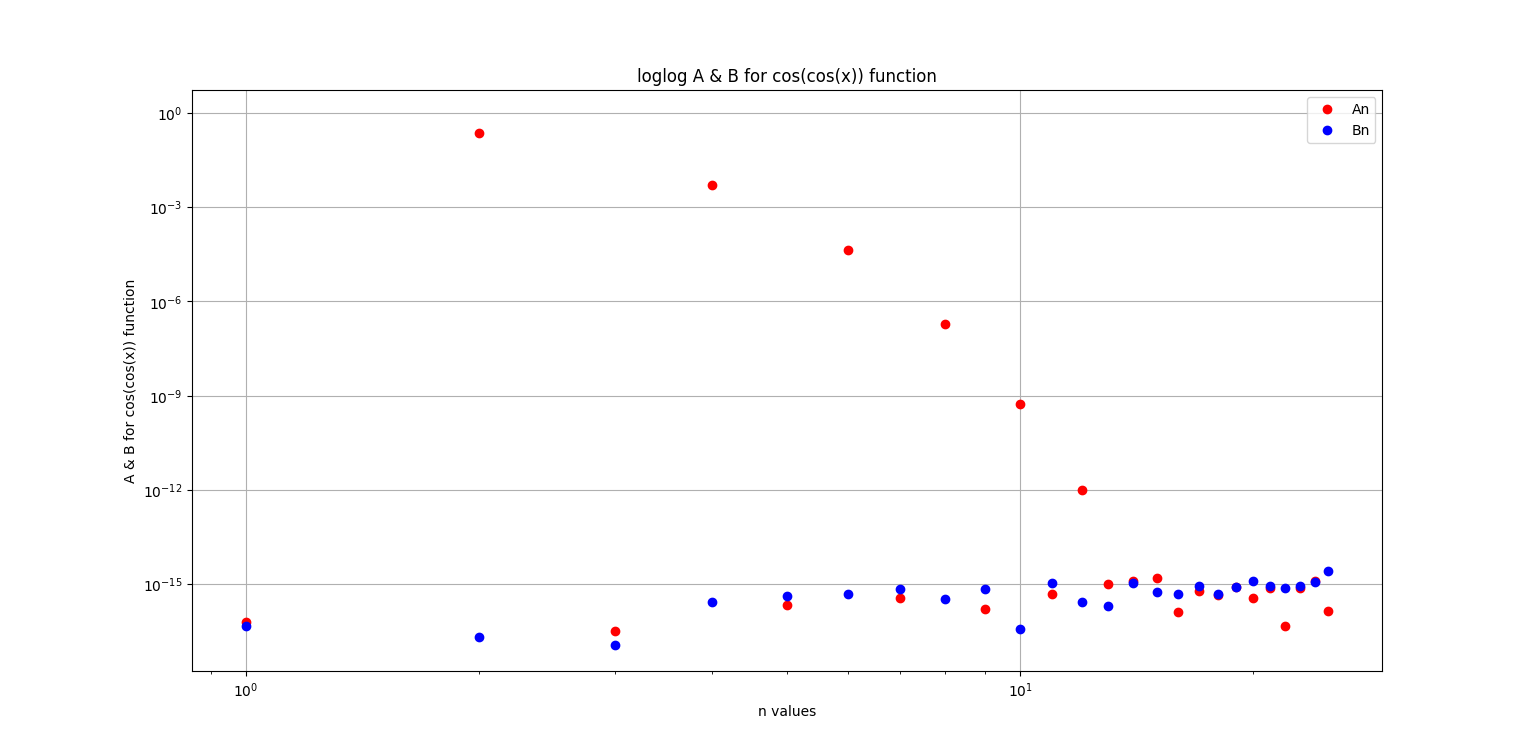
\includegraphics[height=12cm]{Figure_6.png}
\label{fig:exemplo}
\end{figure}
 Compared to the first plot and the magnitude is greatly improved. But we still have a peak that is two samples wide. But that is because $\sqrt{2}$ lies between 1 and 2, which are the two fourier components available. So, using four times the number of points would give promising results. As at that time $\sqrt{2}$ is not in between 1.25 and 1.5.
 
 
\newpage
This is the spectrum of $\sin(\sqrt{2}t)$ with time period $8\pi$-
\begin{figure}[h!]
\centering
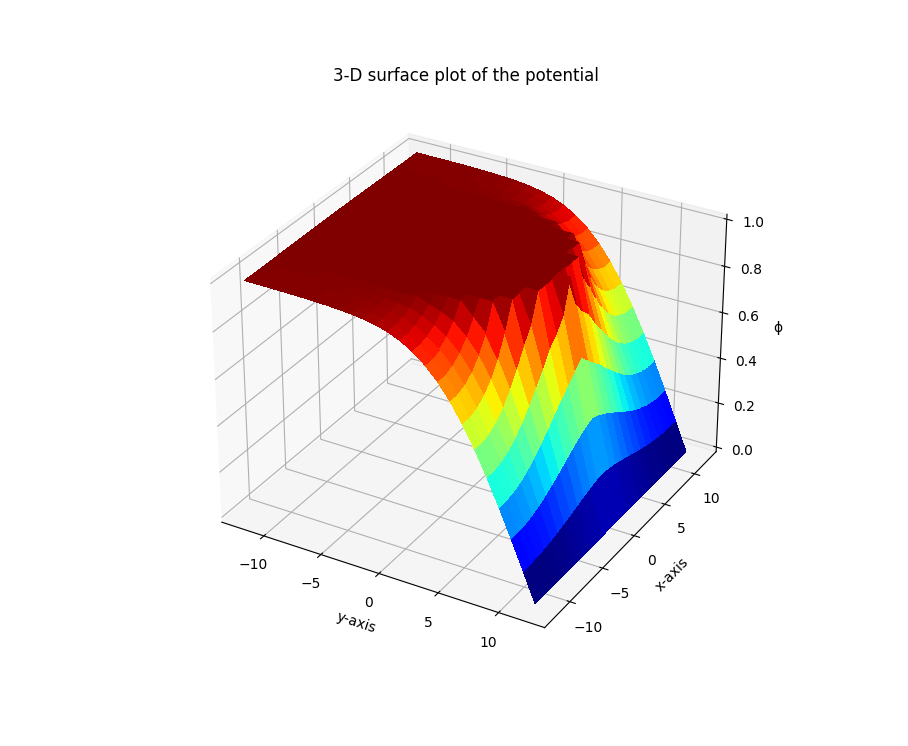
\includegraphics[height=12cm]{Figure_7.png}
\label{fig:exemplo}
\end{figure}

Thus, we get an improved graph which is the result of windowing and choosing right number of points.

\newpage
\section*{Question: 2}
The FFT of $cos^3(0.86t)$ without Hamming window
\begin{figure}[h!]
\centering
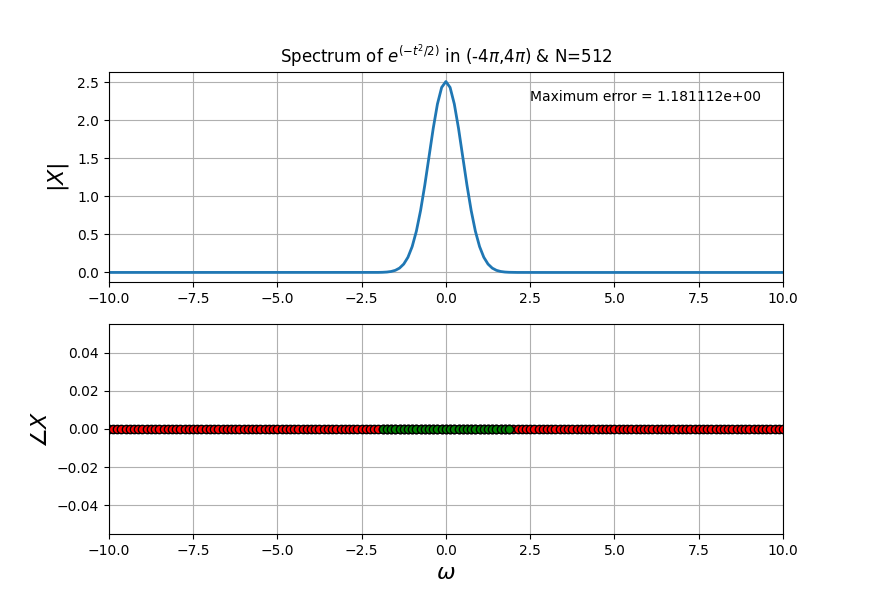
\includegraphics[height=8.3cm]{Figure_8.png}
\label{fig:exemplo}
\end{figure}

The FFT of $cos^3(0.86t)$ with Hamming window
\begin{figure}[h!]
\centering
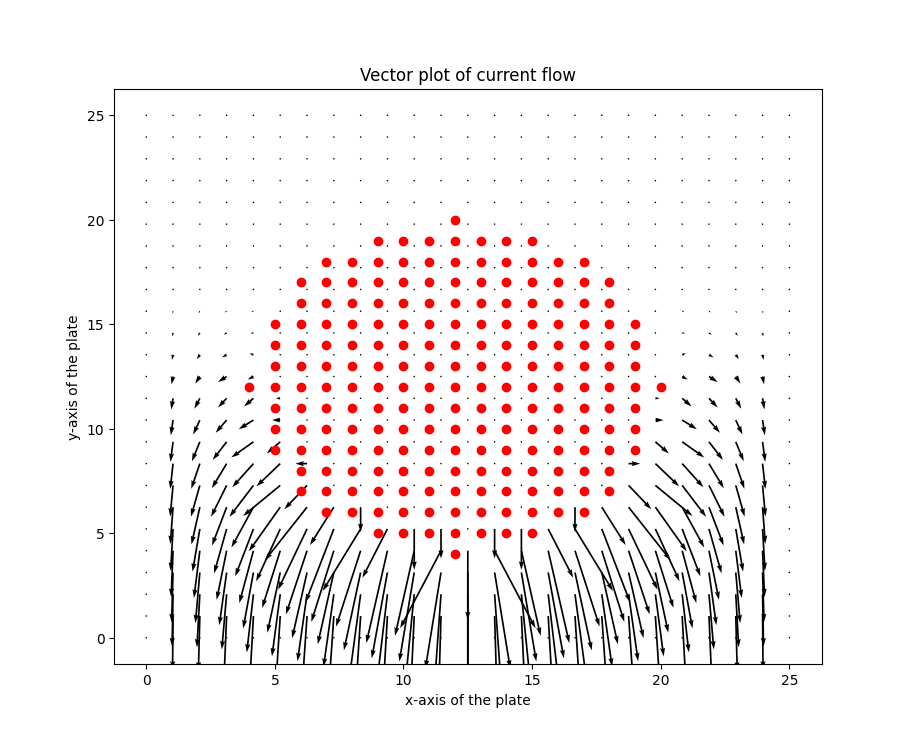
\includegraphics[height=8.3cm]{Figure_9.png}
\label{fig:exemplo}
\end{figure}

Here we can clearly notice that after windowing, the higher frequencies are attenuated and hence the peaks are sharper now.

\newpage
\section*{Question: 3}
Now from $cos(\omega t + \delta)$ signal, we take 128 samples in time range of $-\pi$ to $\pi$ , with 0.5$<$ $\omega_{0}$ $<$ 1.5 
\\Here is the Spectrum of $cos(1.5 t + 0.5)$-
\begin{figure}[h!]
\centering
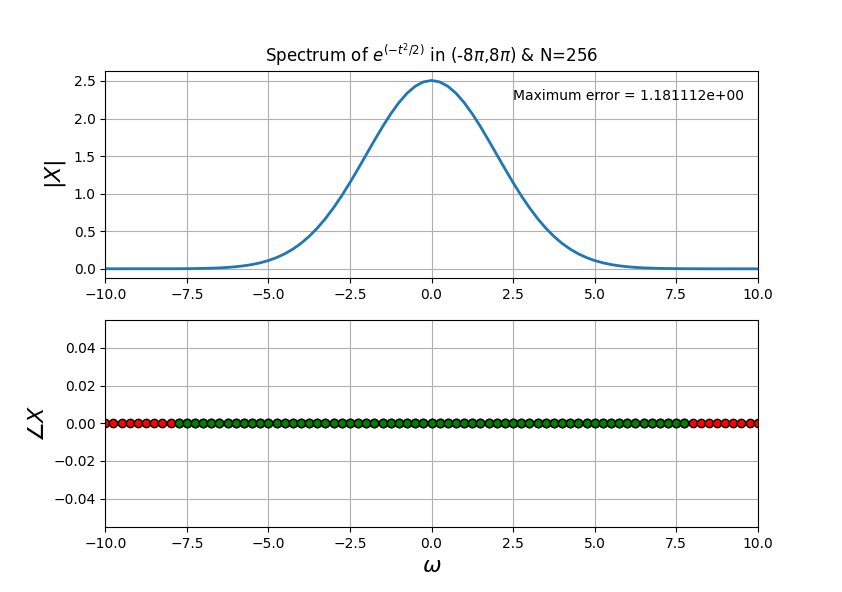
\includegraphics[height=10cm]{Figure_10.png}
\label{fig:exemplo}
\end{figure}

From the signal we find the two peaks at $\pm$ $\omega_{0}$. And estimate $\omega$ using weighted average and $\delta$ by a window on each half of $\omega$. And we get-
\begin{equation}
  \begin{aligned}
    \omega_{0} = 1.5163\\
    \delta = 0.5068
  \end{aligned}
\end{equation}

\newpage
\section*{Question: 4}

Now, we repeat the same above process but now we add noise to the signal and windowing it too.
\\Here is the Spectrum of $cos(1.5 t + 0.5)$ with Hamming windowing and added Noise-
\begin{figure}[h!]
\centering
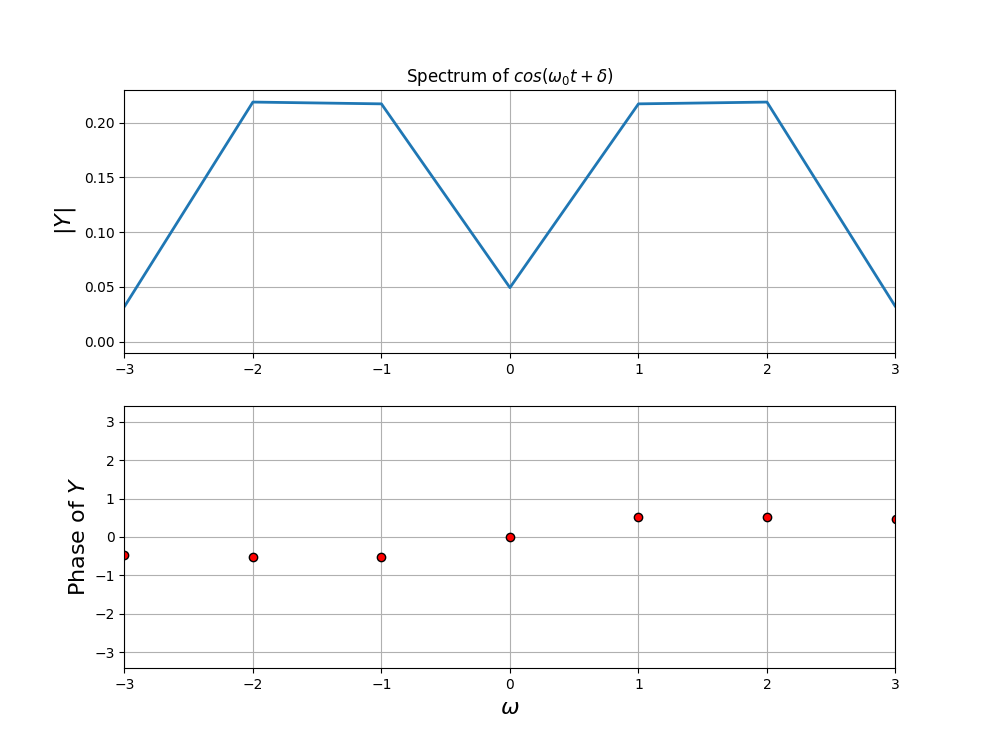
\includegraphics[height=10cm]{Figure_11.png}
\label{fig:exemplo}
\end{figure}

Same as the previous time, from the signal we find the two peaks at $\pm$ $\omega_{0}$. And estimate $\omega$ using weighted average and $\delta$ by a window on each half of $\omega$. This time we get-
\begin{equation}
  \begin{aligned}
    \omega_{0} = 2.0530\\
    \delta = 0.5038
  \end{aligned}
\end{equation}

\newpage
\section*{Question: 5}

Here we will be plotting DFT of Chirped signal function-
\begin{equation*}
f(t)=cos(16t(1.5+\frac{t}{2\pi}))
\end{equation*}
for t going from −$\pi$ to $\pi$ in 1024 steps, while frequency continuously changes from 16 to 32 radians per second. 
\\Here is the Spectrum of windowed Chirped function-
\begin{figure}[h!]
\centering
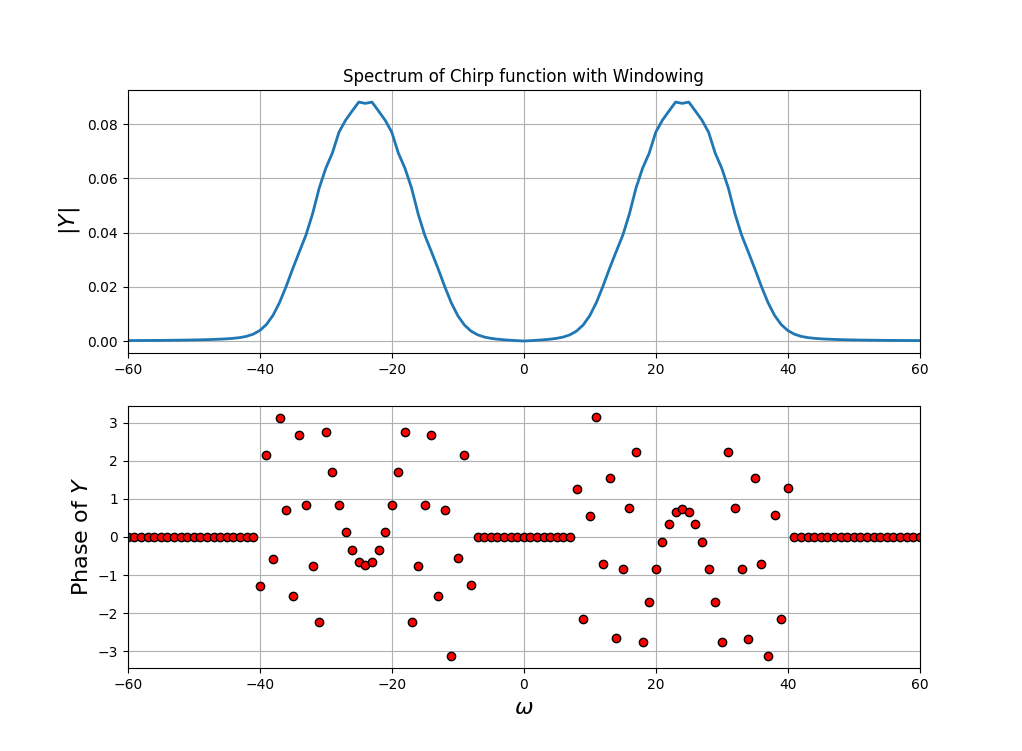
\includegraphics[height=12cm]{Figure_12.png}
\label{fig:exemplo}
\end{figure}

Same as the previous time, we will find $\omega_{0}$ and $\delta$ for this windowed Chirped function and we get-
\begin{equation}
  \begin{aligned}
    \omega_{0} = 24.0084\\
    \delta = 1.6044
  \end{aligned}
\end{equation}

\newpage
Similarly, here is the Spectrum of Non-windowed Chirped function-

\begin{figure}[h!]
\centering
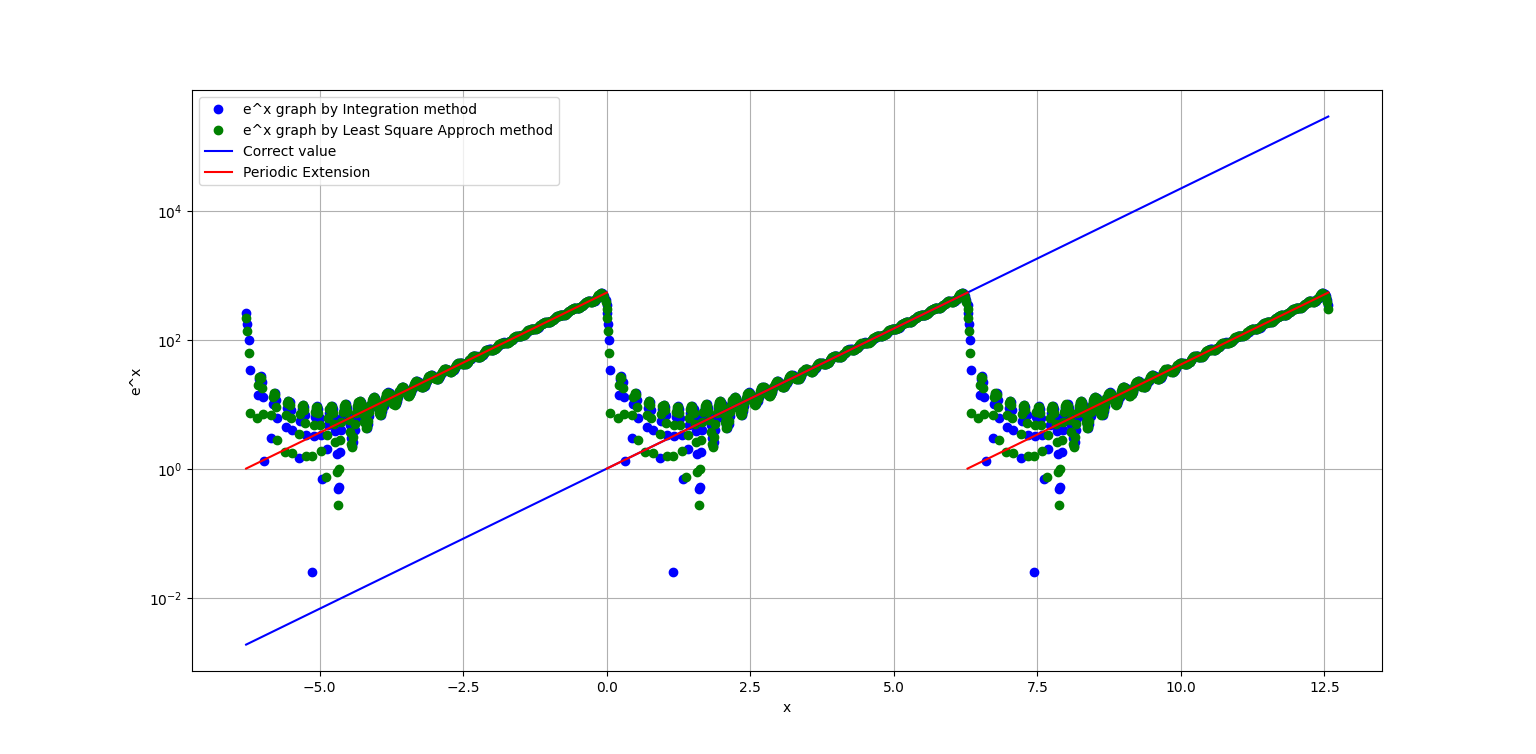
\includegraphics[height=12cm]{Figure_13.png}
\label{fig:exemplo}
\end{figure}

Same as the previous time, we will find $\omega_{0}$ and $\delta$ for this Non-windowed Chirped function and we get-
\begin{equation}
  \begin{aligned}
    \omega_{0} = 24.5193\\
    \delta = 1.3646
  \end{aligned}
\end{equation}

\newpage
\section*{Question: 6}

From the same chirped signal, now we will break the 1024 vector into pieces that are 64 samples wide. And then extract the DFT of each and store as a column in a 2D array. Then plot the array as a surface plot to show the variation of Frequency vs. Time.\\\\
Here is the Magnitude surface plot of Fragmented Chirped siganl-

\begin{figure}[h!]
\centering
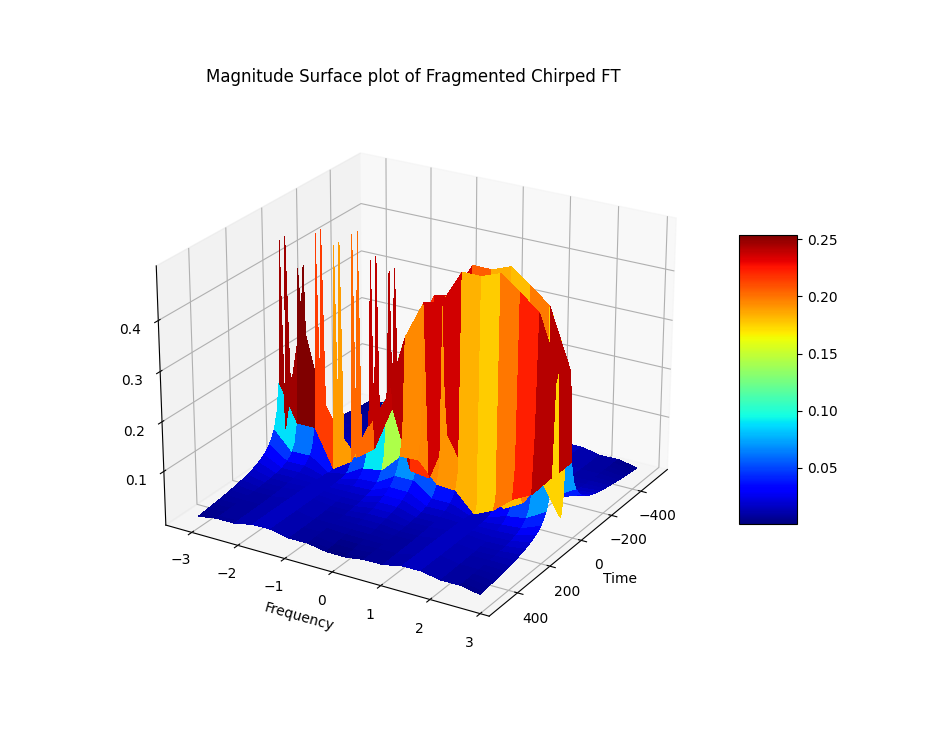
\includegraphics[height=16cm]{Figure_14.png}
\label{fig:exemplo}
\end{figure}

\newpage
Here is the Phase surface plot of Fragmented Chirped siganl-
\begin{figure}[h!]
\centering
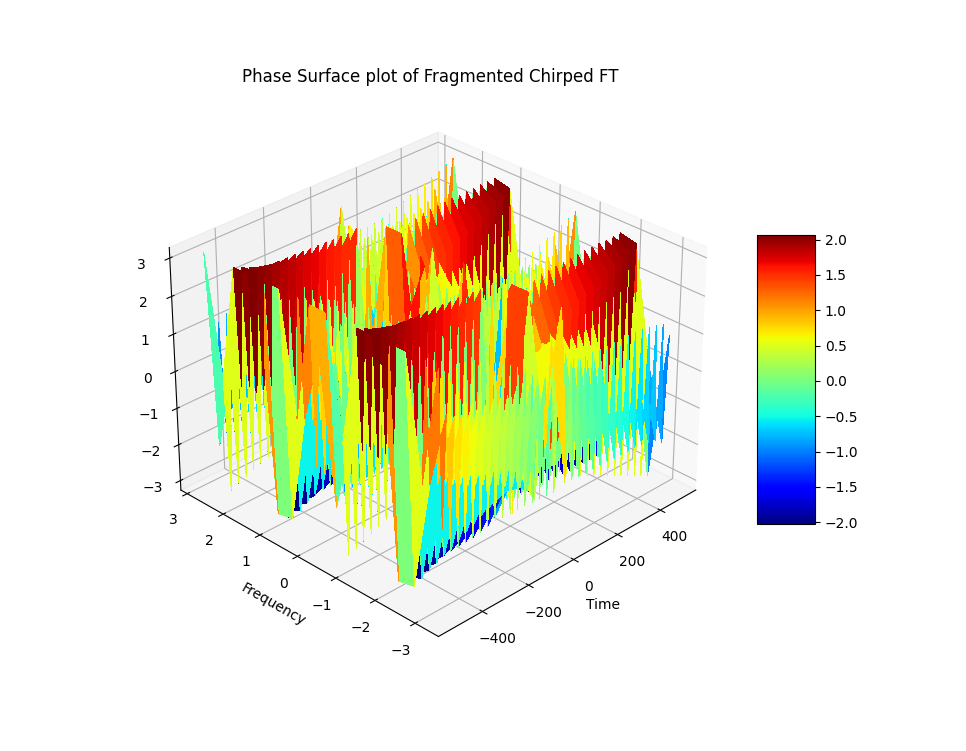
\includegraphics[height=14cm]{Figure_15.png}
\label{fig:exemplo}
\end{figure}

\section*{\textbf{Conclusion:}}
We can plot and analysis precise DFT of Non-periodic signal in Python. Thus, we learnt a lot of interesting things in this assignment, and proving once again that Python is compatible with various signal processing problems.

\begin{center} 
\textbf{Thank you!}
\end{center} 
\end{document}
